% !TeX spellcheck = en_US
% !TeX root = ./0_article.tex

\section{Introduction}
%\IEEEPARstart{S}{everal} researches have studied Body Biasing Injection (BBI) in the past few years.
%While this injection method had been \textcolor{orange}{paused/forgotten} for a few years, it has recently regained some interest.
%Among the latest studies, a modeling and simulation flow has been proposed, alongside better platforms allowing to achieve greater reproducibility and a deeper analysis of the mechanisms at works in digital integrated circuits subjected to BBI.
%In addition to that

%	\subsection{Context}
	\IEEEPARstart{N}{owadays}, electronic devices are found in every economic sector, and very often manipulate sensitive and confidential data, such as in bank transactions, Internet of Things (IoT) devices, smartcards, or smartphones.
	To ensure data authenticity and confidentiality, these devices embed cryptographic algorithms.
	While theoretically secure and robust, once implemented on actual devices, these algorithms become fallible by leaking parts of the manipulated data through various physical quantities such as electromagnetic waves, infrared emissions, or sound emissions, not to cite them all.
	In addition to this, they are sensitive to external disturbances.

	Cybersecurity, more specifically hardware security, takes place in this context
%	In this context, cybersecurity takes place, more specifically hardware security.
	When comes hardware security often comes side-channel attacks and fault injection attacks.
	On the one hand, side-channel attacks take advantage of the circuit leakage by measuring the various physical quantities available.
	On the other hand, fault injection aims at inducing physical disturbances into circuits, with methods like Electromagnetic Fault Injection (EMFI) \cite{mathieuEMFIFirst, mathieuEMFI}, Laser Fault Injection (LFI) \cite{lfiFaultModel}, or Body Biasing Injection (BBI) \cite{bbiOrigin}, not to cite them all.
	Among these methods, EMFI and LFI are widely studied and understood.
	However, despite a resurgence in the past few years, BBI knowledge is still less mature compared to the previously cited methods.
	Therefore, this article is dedicated in presenting our work on Body Biasing Injection.

%	\IEEEPARstart{W}{hen} working with cybersecurity, more specifically with hardware security, involving various integrated circuits ranging from smartcards, smartphones, or microcontrollers, various fault injection methods are often considered.
%	We can point out some of the most documented methods such as Electromagnetic Fault Injection (EMFI) \cite{mathieuEMFIFirst, mathieuEMFI}, Laser Fault Injection (LFI) \cite{lfiFaultModel}, or Body Biasing Injection (BBI) \cite{bbiOrigin}, not to cite them all.
%	Our work is dedicated in studying Body Biasing Injection.



	\subsection{Fault injection objectives}
		Before going further in the discussion about BBI, let us first outline the main objectives of fault injection methods.
		Most commonly, they are set up to perform various malicious manipulation on integrated circuits, such as:
		\begin{itemize}
			\item Denial of service (DoS) \textrightarrow\ Stop circuit operation and the related services;
			\item Verification bypass \textrightarrow\ Modify data on the fly to fake authenticity (e.g. to bypass bootloader security);
			\item Confidential data extraction \textrightarrow\ Modify data to perform differential fault analysis.
		\end{itemize}
		To perform these objectives, we can use various injection methods, such as EMFI, LFI or BBI.
		Before presenting our work on BBI further, let us analyze the available and existing BBI platforms in the state-of-the-art.
%		\textcolor{red}{To finish.}

	\subsection{BBI in the state-of-the-art}
%		\textcolor{red}{Fait-on un paragraphe sur les plateformes industrielles comme dans la thèse ? Je trouve ça encombrant.}
%
		When compared to EMFI, BBI has a smaller state-of-the-art, whether in the amount of scientific papers published or in the amount of industrial platforms proposed.
		Currently, there are ten main works lingering on BBI \cite{bbiOrigin, bbiSecond, bbiThird, bbiColin,japbbi, japbbi2, mybbiCosade, mybbiFdtc2022, mybbifdtc2023, colinFdtc2023}.
		Each one of them made a unique contribution for a better understanding of BBI.

		The first one \cite{bbiOrigin} introduced the technique and presented a Bellcore attack on the targeted IC.
		Then, one year later, another work \cite{bbiSecond} further studied the method, followed by a third work three years later \cite{bbiThird}, introducing an advanced test bench to work and perform attacks with BBI.
		After that, another work presented a low-cost BBI platform, dedicated to WLCSP devices \cite{bbiColin}.
		Then, quite interestingly researchers proposed a study of BBI using an ESD gun as a voltage surge generator \cite{japbbi, japbbi2}.
		At the same time, the impact of substrate thickness on BBI efficiency has been studied in \cite{mybbiCosade}, in addition to a simulation flow and better practices \cite{mybbiFdtc2022,mybbifdtc2023}.
		Eventually, one last work proposed a safety-focused low-cost and open-source design for the practice of BBI \cite{colinFdtc2023}.
%		\textcolor{red}{To FINISH.}

		However, despite this extensive work, there are still unanswered questions, and the current works aims at bringing more answers thanks to a compilation of our work on Body Biasing Injection.

		Before going any further, let us introduce the platform we use for the present work.

%		Before introducing the present work, let us eventually analyze the industrial platforms proposed by various manufacturers and introduce our own test platform.
%		We can distinguish three major actors proposing BBI related products:
%		\begin{itemize}
%			\item Langer EMV-Technik;
%			\item Riscure;
%			\item NewAE Technology.
%		\end{itemize}
%
%		% !TeX spellcheck = en_US
% !TeX root = ./0_article.tex

\begin{figure}
	\centering
	\subfloat[][Langer]{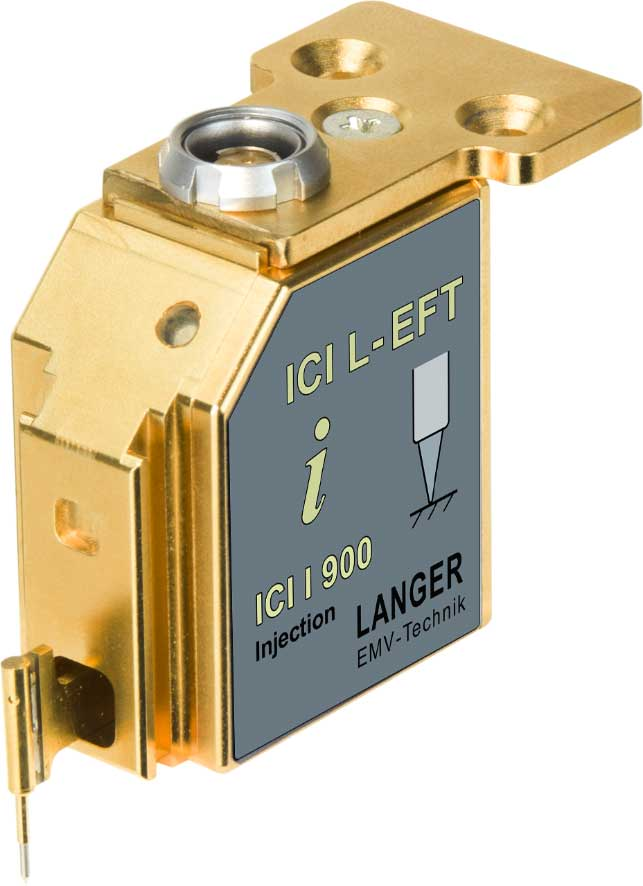
\includegraphics[width=0.2\columnwidth]{./figures/langerBBI.jpg}}
	\hspace{0.1\columnwidth}
	\subfloat[][Riscure]{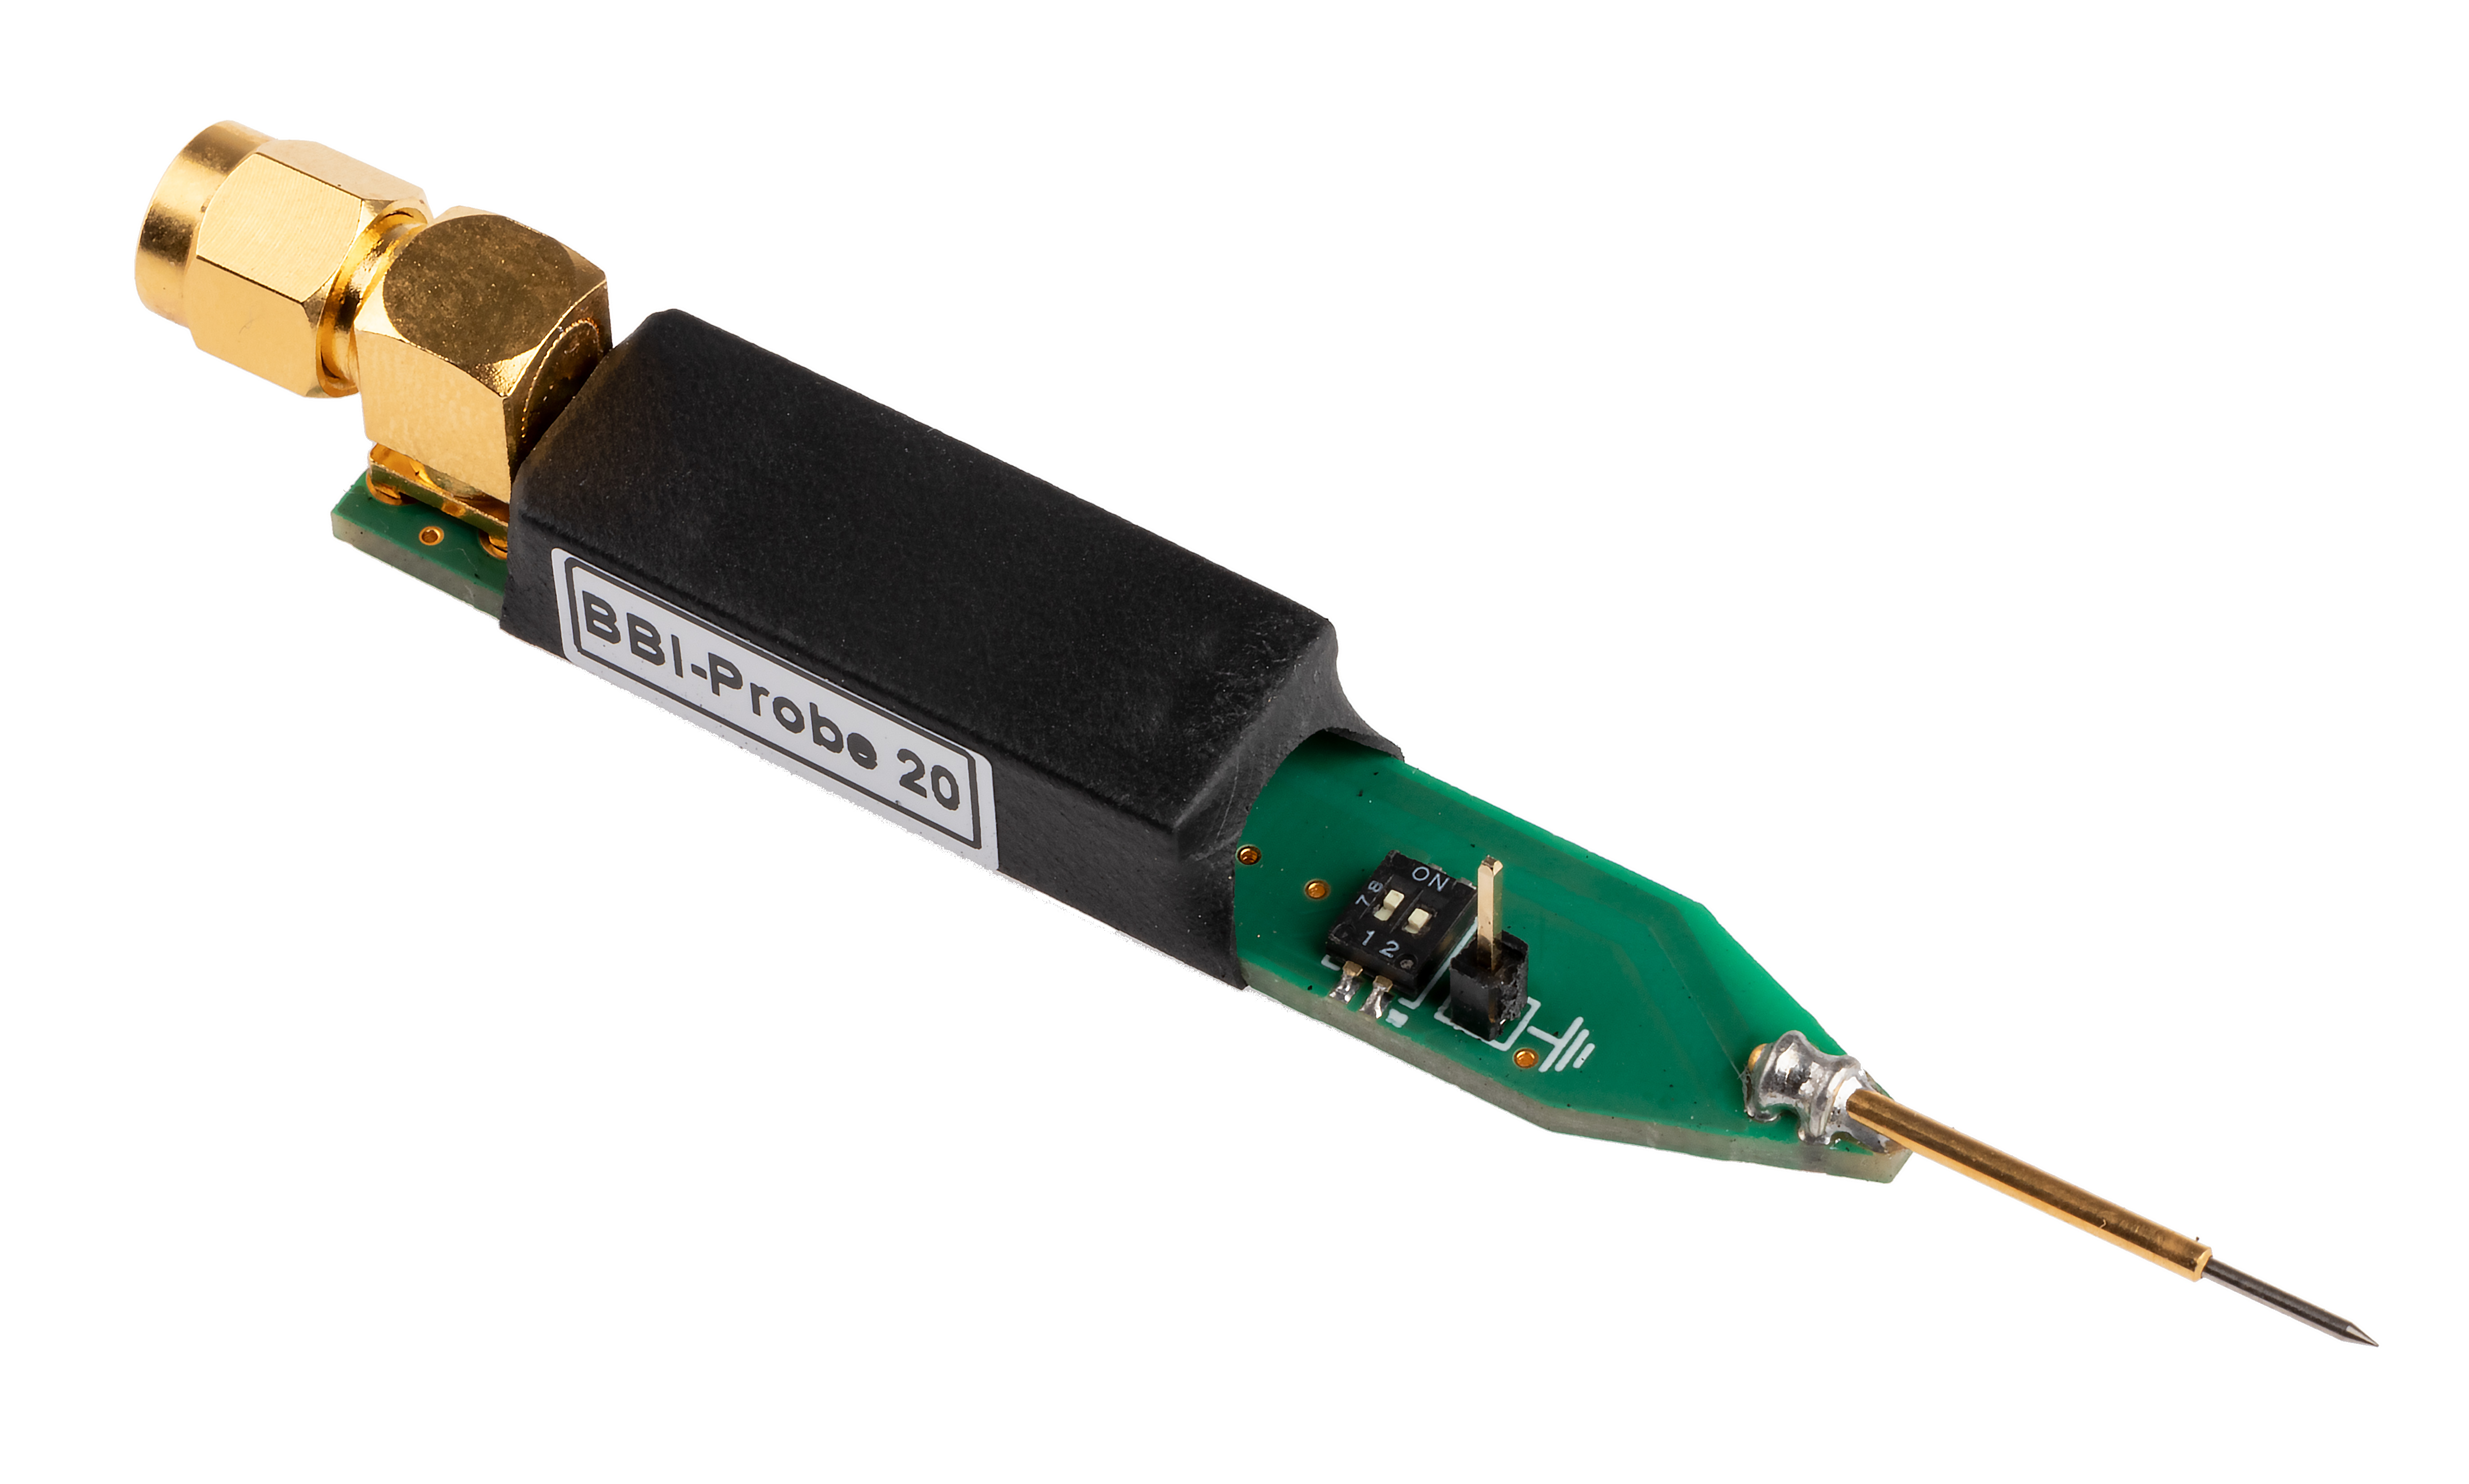
\includegraphics[width=0.425\columnwidth]{./figures/em-fi-bbi-probe-20-black.jpg}}
	\caption{Langer and Riscure BBI probes.}
	\label{riscure_langer}
\end{figure}
%		\subsubsection{Langer EMV-Technik platform}
%			The German society Langer EMV-Technik proposes an all-in-one and ready-to-use BBI platform composed of two hardware tools:
%			\begin{itemize}
%				\item A current pulse generator with a metal needle, shown in Fig. \ref{riscure_langer}.a;
%				\item A general controller called "Burst Power Station", combining a power supply, control and monitor tool and a software.
%			\end{itemize}
%
%		\subsubsection{Riscure BBI platform}
%			Similar to Ledger, Riscure proposes a complete BBI platform.
%			It is made of two major tools: a generator, originally designed for EMFI probes, and a set of four probes.
%			One of the probes is shown in Fig. \ref{riscure_langer}.b.
%			The generator is a voltage pulse one................................................

	\subsection{Our BBI platform}
		As the commercial platforms, our platform is focused on two main pieces of equipment: a voltage pulse generator and a metallic probe.

		The generator model is the AVRK-4-B from the society Avtech Electrosystems Ltd.
		This model is commonly used for EMFI, but is suitable for BBI, and its specifications are the following:
		\begin{itemize}
			\item Pulse amplitude: \textpm\ [150, 750] V;
			\item Pulse width: [6, 20] ns;
			\item First edge rise/fall time: 4 ns;
			\item Second edge rise/fall time: load dependent;
			\item Recovery time: \textless\ 1 ms;
			\item Propagation delay (PD): 150 ns;
			\item Jitter: \textpm\ 100 ps \textpm\ 0.03 \% of PD;
			\item DC-coupled output;
			\item Loaded with 50 \textOmega.
		\end{itemize}
		% !TeX spellcheck = en_US
% !TeX root = ./0_article.tex

\begin{figure}
	\centering
	\subfloat[][Global view]{\includegraphics[width=0.4\columnwidth]{./figures/sondeBBI_loin_raw.png}}
	\hspace{0.1\columnwidth}
	\subfloat[][Zoomed view]{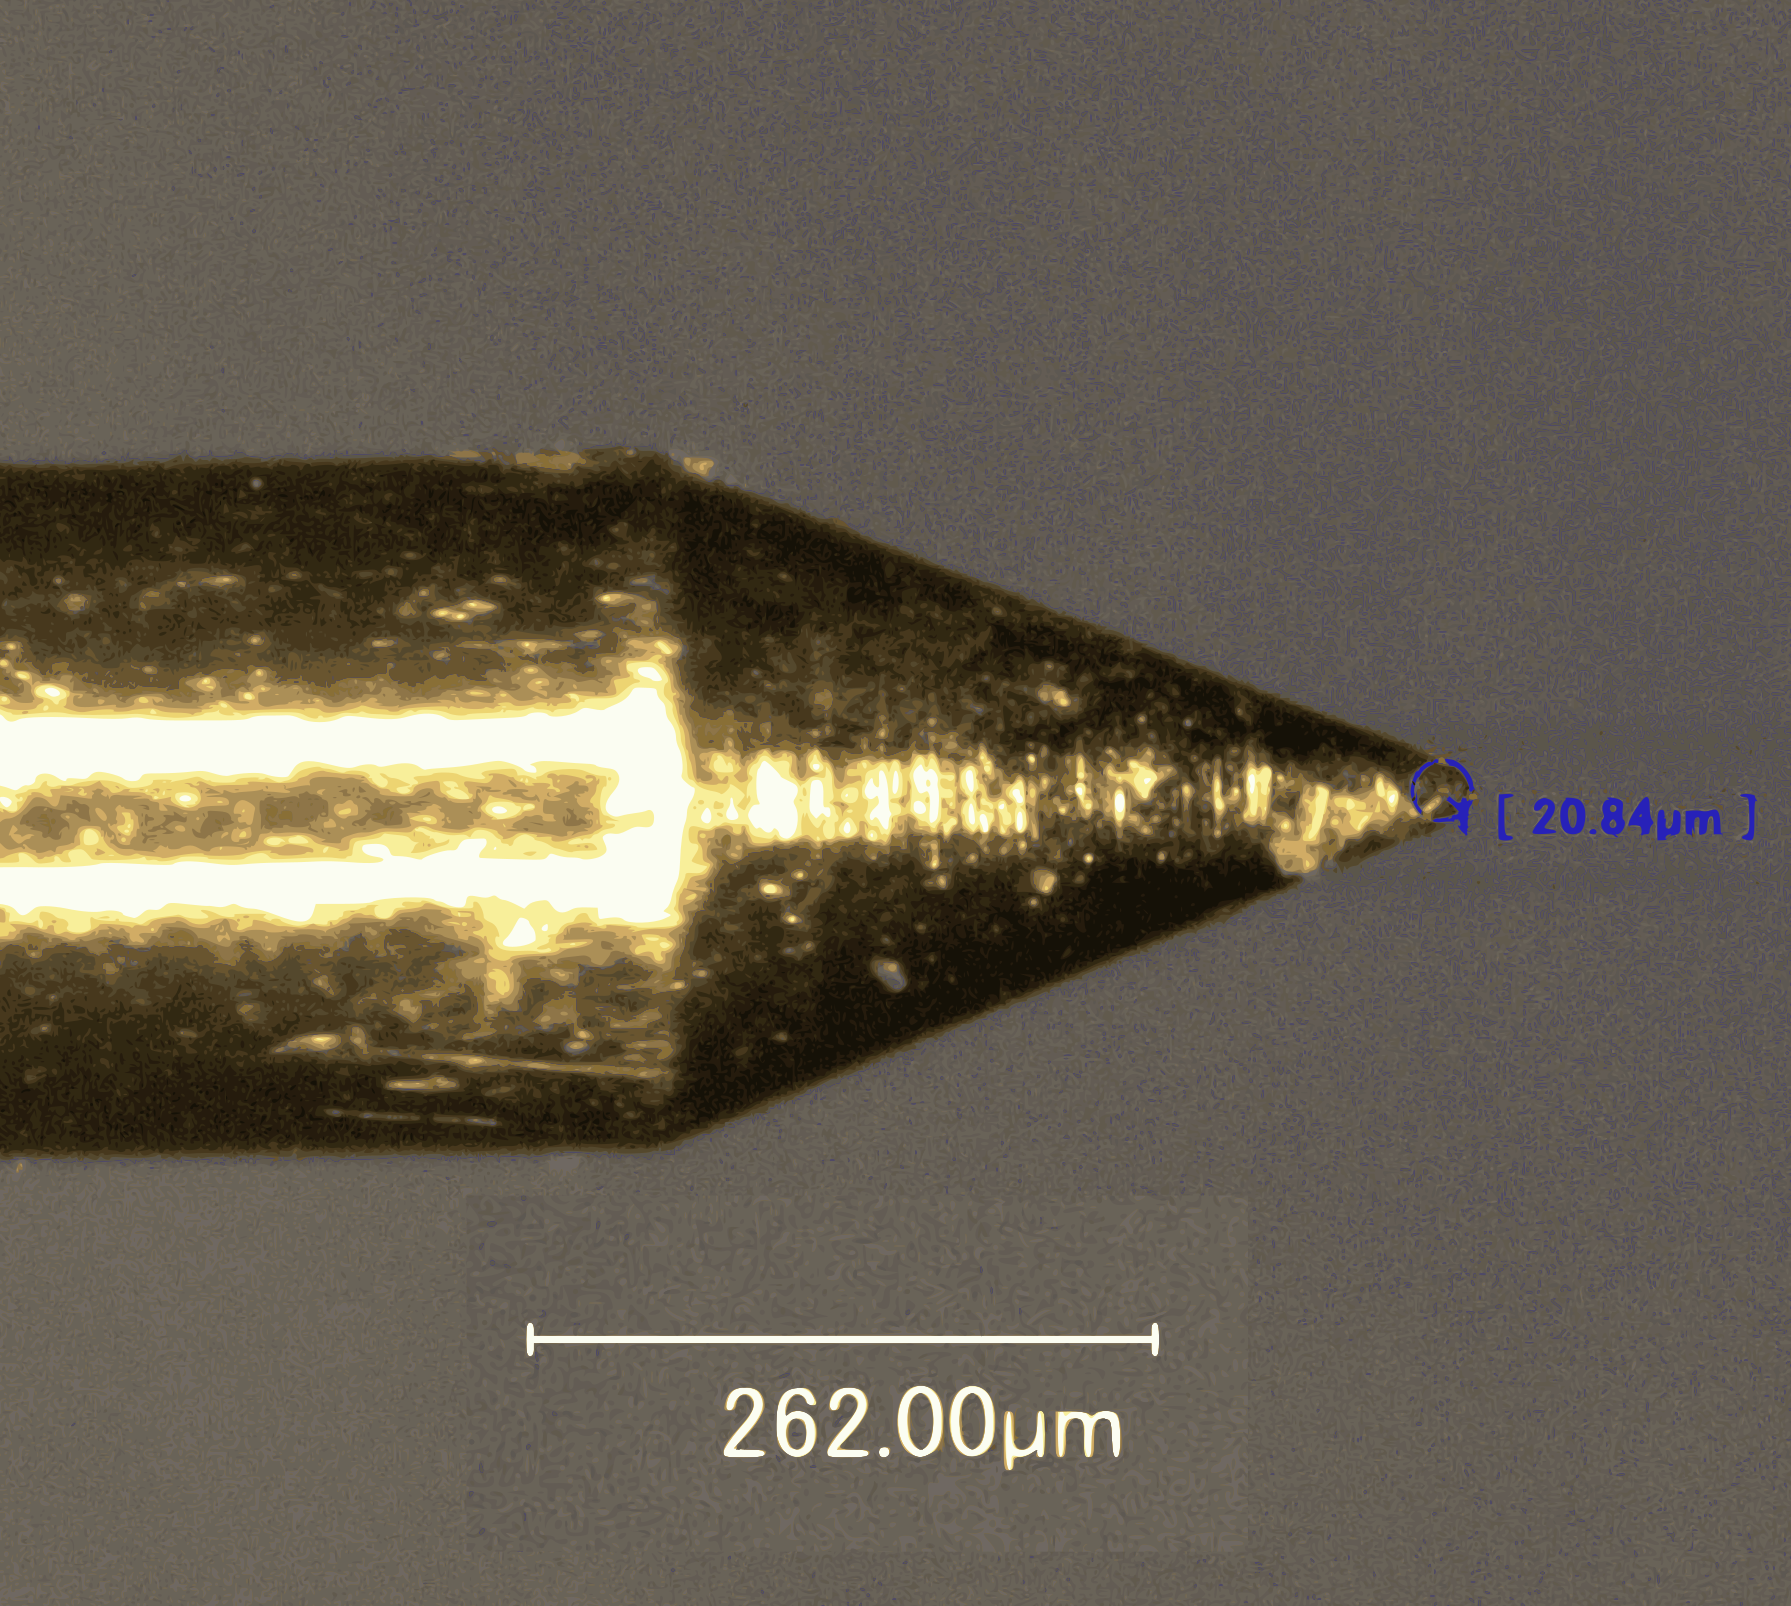
\includegraphics[width=0.4\columnwidth]{./figures/pointeBBI2.png}}
	\caption{Our custom BBI probe.}
	\label{bbi_probe}
\end{figure}
		Probably the most distinctive piece of equipment when it comes top BBI is the probe.
		Some BBI probes can be active, others passive and less expensive.
		However, it is important to keep this piece of equipment relatively cheap as it endures most of the physical strain on a BBI platform, and should be easy to replace or repair.
		Fig. \ref{bbi_probe} shows two pictures of our probe from different angles.
		The one we use is custom made around three parts:
		\begin{itemize}
			\item A spring-loaded metallic tip, with a 20 \textmu m head diameter;
			\item A SMA connector, where the tip is soldered;
			\item A custom 3D-printed enclosure holding the pieces together and cheap to replace.
		\end{itemize}
		The spring-loaded tip is 17 mm long and has a global diameter of 0.635 mm.
		It is specified for a 1.5 A nominal current, and its electrical resistance measures around 70 m\textOmega.
		The total cost of the probe is of 20 \texteuro.

	\subsection{BBI interrogations}
%		With all the work in the state-of-the-art in mind, there are still remaining questions unanswered about BBI, such as:
		With all the work in the state of the art in mind, we will try to bring more answers on various points such as:
		\begin{itemize}
			\item How to increase the reliability and repeatability of BBI experiments?
			\item How to model large scale circuits under BBI?
			\item How BBI induced faults occur?
		\end{itemize}
		We will answer these questions through the next section of this work.
